%%%%%%%%%%%%%%%%%%%%%%%%%%%%%%%%%%%%%%%%%%%%%%%%%%%%%%%%%%%%%%%%%%%%%%
% Based on LaTeX Template: Newsletter  
% Source: http://www.howtotex.com
%
% Adapted for Nebraska Ornithologists' Union Burrowing Owl
% 
%%%%%%%%%%%%%%%%%%%%%%%%%%%%%%%%%%%%%%%%%%%%%%%%%%%%%%%%%%%%%%%%%%%%

% important things to run first

% use lualatex

%!TEX program = lualatex

%% Tag PDF for accessibility

\DocumentMetadata{
	lang        = en,
	pdfstandard = ua-2,
	pdfstandard = a-4f, %or a-4
	tagging     = on
} 

\documentclass[10pt,letterpaper]{article}

%%% ---------------
%%% PREAMBLE
%%% ---------------


% Define geometry (without using the geometry package)
\setlength\topmargin{-48pt}
\setlength\headheight{0pt}
\setlength\headsep{25pt}
\setlength\marginparwidth{-20pt}
\setlength\textwidth{7.0in}
\setlength\textheight{9.5in}
\setlength\oddsidemargin{-30pt}
\setlength\evensidemargin{-30pt}

% references

% packages for references
\usepackage[backend=biber, 
	%%%% use below line for numeric citations %%%%%			style=numeric-comp, % style compresses, orders in text citations
	style=authoryear-comp, % author year citation style
	dashed = false, %doesnt dash the same author in reference list
	sorting=nyt, % within bibliography by name, year, then title
	maxbibnames=99,% prints up to 99 names in bibliography
	mincitenames = 1,
	maxcitenames = 2,
	uniquename = false,
	uniquelist = false]{biblatex} %reduces number of possible in text citations to a max of 2, otherwise does et al.
\addbibresource{newsletter.bib}

\AtEveryBibitem{
	\clearfield{url}
	\clearfield{issn}
	\clearfield{urlyear}
	\clearlist{language}
	\clearfield{month}
	\clearfield{note}
	\clearname{editor}
	\clearfield{eprint}
}

% remove "in" from citations
\renewbibmacro{in:}{}

% remove "pages" from bibliography
\DefineBibliographyStrings{english}{%
	page             = {},
	pages            = {},
} 

% add ":" before pages
\renewcommand{\postnotedelim}{\addcolon}

\setlength{\parindent}{36pt}

% remove double spacing after periods
\frenchspacing

\usepackage[english]{babel}			% english
\usepackage{graphicx}				% images
\usepackage{amssymb,amsmath}		% math
\usepackage{multicol}				% three-column layout
\usepackage{url}				% URL package
\usepackage{marvosym}				% symbols
\usepackage{wrapfig}				% wrapping text around figures
\usepackage[T1]{fontenc}			% font encoding
\usepackage{charter} 				% Charter font for main content
\usepackage{blindtext}				% dummy text
\usepackage{datetime}				% custom date
\newdateformat{mydate}{\monthname[\THEMONTH] \THEYEAR}

\usepackage[pdfpagemode=FullScreen,
			colorlinks=true,
			linkcolor=blue]{hyperref}	% links and pdf behaviour
\hypersetup{colorlinks = true, % make links different color
	pdfcreator         = {Jacob C. Cooper}, % document creator
	linkcolor          = black, % links within document "hidden"
	citecolor          = blue, % links to citations blue
	urlcolor           = blue} % links to web pages blue
	
% Customize (header and) footer
\usepackage{fancyhdr}
\pagestyle{fancy}
\lfoot{	\footnotesize 
		Burrowing Owl \\
		\Mundus\ \href{https://noubirds.org/}{NOUbirds.org}	\quad
		% \Telefon\ 555-5555											\quad
		%\Letter\ \href{mailto:frits@howtotex.com}{frits@howtotex.com}
	  }
\cfoot{}
\rfoot{\footnotesize ~\\ Page \thepage}
\renewcommand{\headrulewidth}{0.0pt}	% no bar on top of page
\renewcommand{\footrulewidth}{0.4pt}	% bar on bottom of page

%%% ---------------
%%% DEFINITIONS
%%% ---------------

% Define separators
\newcommand{\HorRule}[1]{\noindent\rule{\linewidth}{#1}} % Creating a horizontal rule
\newcommand{\SepRule}{\noindent							 % Creating a separator
						\begin{center}
							\rule{250pt}{1pt}
						\end{center}
						}						

% fonts
\usepackage{fontspec}
%\newfontfamily{\lexend}{Lexend}
% \DeclareTextFontCommand{\cwy}{\cherokeefam}

%\setmainfont{CrimsonText}[
%	Path=../Fonts/Crimson/,
%	Extension=.ttf,
%	UprightFont=*-Regular,
%	BoldFont=*-Bold,
%	ItalicFont=*-Italic,
%	BoldItalicFont=*-BoldItalic,
%]

% Define Title en News input
\newcommand{\JournalName}[1]{%
		\begin{center}	
			\Huge \fontspec{QTBrushStroke}
			%\usefont{T1}{QTBrushStroke}{m}{n}
			#1%
		\end{center}	
		\par \normalsize \normalfont}
		
\newcommand{\JournalIssue}[1]{%
		\hfill \textsc{\mydate \today, No #1}
		\par \normalsize \normalfont}

\newcommand{\NewsItem}[1]{%
		% \usefont{T1}{augie}{m}{n} 	
		\fontspec{QTBrushStroke}
		\large #1 \vspace{4pt}
		\par \normalsize \normalfont}
		
\newcommand{\NewsAuthor}[1]{%
			\hfill by \textsc{#1} \vspace{4pt}
			\par \normalfont}		


% for fancy big letters
\usepackage{lettrine}

\usepackage{lipsum}

%%% ---------------
%%% BEGIN DOCUMENT
%%% ---------------
\begin{document}
% Title	
% -----
\JournalIssue{1}
\JournalName{Burrowing Owl}
\noindent\HorRule{3pt} \\[-0.75\baselineskip]
\HorRule{1pt}
% -----

% Front article
% -----
\vspace{0.5cm}
	\SepRule
\vspace{0.5cm}

\begin{center}
\begin{minipage}[h]{0.75\linewidth}
	\begin{wrapfigure}{l}{0.41\textwidth}
		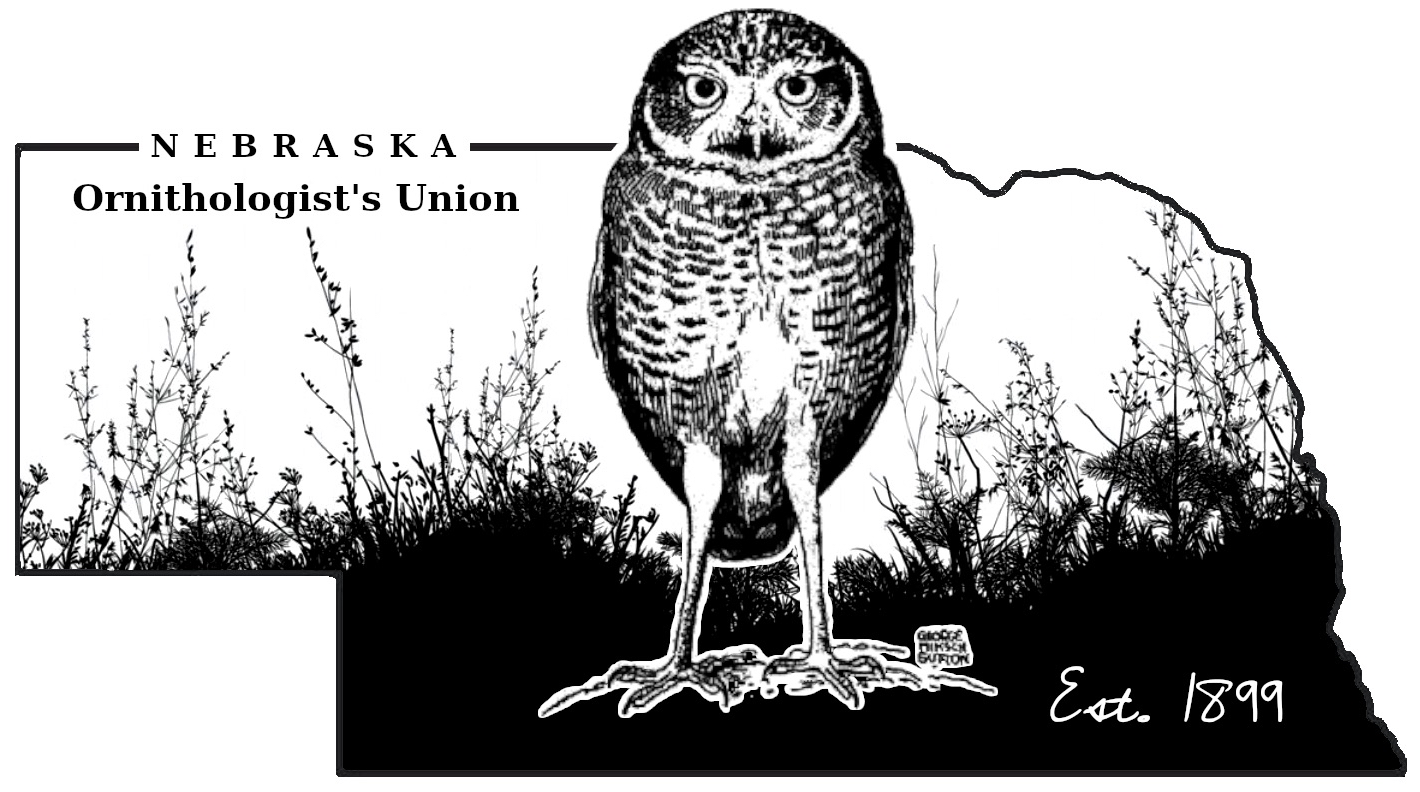
\includegraphics[width=0.42\textwidth,alt={The logo for the Nebraska Ornithologists' Union.}]{../logo/nou_logo.png}
		\\	% this spacer is needed to make the text on the right fit OK
	\end{wrapfigure}
	
	\NewsItem{From the President's Desk}
	\lettrine{F}{ew} would have guessed how spring migration was going to play out for us this year. Well, it was pretty dope. \lipsum[1]
	%\emph{\blindtext}
\end{minipage}
\end{center}
% -----


% Main matter of the newsletter
% -----
\vspace{0.5cm}
	\SepRule
\vspace{0.5cm}

\section*{Predicting what comes next}
\NewsAuthor{Jacob C. Cooper, Tobin  Brown}

\begin{multicols}{2}
	
	\lettrine{I}{t} is always fun to speculate what will be next in Nebraska, and indeed, we have had the likes of Joel G. Jorgensen, W. Ross Silcock, and Mark Brogie predict what they think will show up in Nebraska in both \colorbox{red}{YEAR and YEAR}. To keep the tradition going, and in light of new (and frankly absurd) weather patterns and additions to the state lists of Nebraska and other plains stats, we thought we should revisit this topic.
	
	\NewsItem{Correct predictions}
	
	In all, we had five correct predictions from the aforementioned folks:
	
	\begin{enumerate}
		\item \textbf{Western Bluebird \textit{Sialia occidentalis}}
	\end{enumerate}
	Predicted by Ross Silcock, this bird was found in extreme southwestern Nebraska within a stone's throw of the Colorado line. While suitable habitat for this species exists not far away in Colorado, the surprising lack of Western Bluebirds in Wyoming and South Dakota indicates that it may be a long time before we get another.
	
	\begin{enumerate}[resume]
		\item \textbf{Limpkin \textit{Araumus guarana}}
	\end{enumerate}
	A pick from Joel G. Jorgensen's `off the wall' picks, a large multi-year irruption of Limpkin from the southeast resulted in Nebraska's first record, as well as double-digit records from Kansas and other nearby states that previously had no records of Limpkin. Research shows that many of these wandering individuals are second year birds with irruptions driven by droughts, and as southeastern populations continue to increase with spreading apple snail (\textit{Pomacea} sp.) populations, there will likely be more Limpkin in Nebraska in the future \parencite{Mutchler02102025}.
	
	\begin{enumerate}[resume]
		\item \textbf{Broad-billed Hummingbird \textit{Cynanthus latirostris}}
	\end{enumerate}
	
	This prediction came true by means of an incredible away-from-feeder migrant found by Caleb Strand in Wilderness Park, \textit{Lancaster}. Incredible, within a few weeks of this record another extralimital individual was found under almost the exact same circumstances in LaBagh Woods, \textit{Cook}, Illinois, making many wonder how many vagrants we miss every year! Given the propensity of this bird to show up in states just south of us, it is likely that another bird will be in Nebraska in the near future.
	
	\begin{enumerate}[resume]
		\item \textbf{Black Phoebe \textit{Sayornis nigricans}}
	\end{enumerate}
	
	The first record of this species came from the southern Panhandle, arguably the one part of the state that looks most like its southwestern desert haunts. This is another species that has been expanding in recent decades, with this species now becoming expected in parts of Colorado where they were wholly absent only 30 years ago. As the climate continues to warm, it seems likely this species will occur in the state again, unless droughts continue to stymie their preferred habitats.
	
	\begin{enumerate}[resume]
		\item \textbf{Fulvous Whistling-Duck \textit{Dendrocygna bicolor}}
	\end{enumerate}
	Formerly the common northern whistling-duck, Fulvous Whistling-Duck has not shown nearly the same ability to spread northwards as its congener, the Black-bellied Whistling-Duck. Despite this, irruptions still do occur, and a flock of these birds in \textit{Lancaster} garnered the first record for the state. Another bird was taken by a hunter in western Nebraska, and, given that the species has nested as far north as Illinois, it seems likely we will be getting this species again.
	
\end{multicols}
	\vspace{0.5cm}
	\NewsItem{Surprise finds}
	While likely discussed, the following species were not in folks' top tens for predicted next species in Nebraska--and it seems very unlikely that Nebraska will get a second record of several of these anytime soon!
	\begin{multicols}{2}
	\begin{enumerate}[resume]
		\item \textbf{Couch’s Kingbird \textit{Tyrannus couchii}}
	\end{enumerate}
	Folks can search their whole lives and not find a first state record for Nebraska, but luck smiled upon Christine Nelson when the first state record of this locally distributed kingbird showed up on her front deck near North Platte!
	
	\begin{enumerate}[resume]
		\item \textbf{Mexican Duck \textit{Anas diazi}}
	\end{enumerate}
	A species likely missing from predictions solely because it wasn't recognized as a species, this taxon has now been definitely recorded from western Nebraska. It seems likely that we will get more records in the future, but possible individuals should be carefully scrutinized for hybrid characters.
	
	\begin{enumerate}[resume]
		\item \textbf{Western Gull \textit{Larus occidentalis}}
	\end{enumerate}
	On the same day as Nebraska's first Westerb Bluebirds was Nebraska's first record of this stunning gull. While not wholly unexpected, it is one of the rare vagrant gulls in interior and eastern North America.
	
	\begin{enumerate}[resume]
		\item \textbf{Black Vulture \textit{Coragyps atratus}}
		\end{enumerate}
		A vagrant of this vulture is not wholly surprising given records in other far-flung regions of North America, and while future records are a certainty, it'll probably be a long wait before we get another in the state.
		
		\begin{enumerate}[resume]
		\item \textbf{Great Kiskadee \textit{Pitangus sulphuratus}}
		\end{enumerate}
		Records in the interior of North America have increased in years, and South Dakota, Kansas, and Colorado now all have records of this stunning tyrant flycatcher.
		
		\begin{enumerate}[resume]
		\item \textbf{Swainson’s Warbler \textit{Limnothlypis swainsoni}}
		\end{enumerate}
		
		
		\begin{enumerate}[resume]
		\item \textbf{Pacific Wren \textit{Troglodytes pacificus}}
		\end{enumerate}
		Another bird likely overlooked because it was considered conspecific with what the Europeans know as \textit{the} wren, recent taxonomic shuffles resulted in both the Winter Wren \textit{T. hiemalis} and the Pacific Wren being split from the Eurasian Wren \textit{T. troglodytes}, and this species was soon thereafter found in Nebraska. A classic example of why we should continue to document and pay attention to distinctive regional subspecies in Nebraska!
		\begin{enumerate}[resume]
		\item Brown Booby
	\end{enumerate}
	\end{multicols}
	
	\NewsItem{Predictions yet to show}
	The following species were predicted in past years, but have yet to show in Nebraska. 
	
	\begin{multicols}{3}
		
	\begin{itemize}
		\item \textbf{Slaty-backed Gull \\ \textit{Larus schistisagus}}
		\item \textbf{Long-billed Murrelet \\ \textit{Syntliboramphus }}
		\item \textbf{Rivoli’s Hummingbird \\ \textit{Eugenes fulgens}}
		\item \textbf{Lesser Nighthawk \\ \textit{Choreiles acutipennis}}
		\item \textbf{Black-backed Woodpecker \\ \textit{Picoides dorsalis}}
		\item \textbf{Woodhouse’s Scrub-Jay \\ \textit{Aphelocoma woodhouseii}}
		\item \textbf{Painted Whitestart \\ \textit{Myioborus pictus}}
		\item \textbf{Fork-tailed Flycatcher \\ \textit{Tyrannus savanna}}
		\item \textbf{Ivory Gull \\ \textit{Pagophila eburnea}}
		\item \textbf{Flammulated Owl \\ \textit{Psiloscops flammeolus}}
		\item \textbf{Gull-billed Tern \\ \textit{Gelochelidon niloctica}}
		\item \textbf{Allen’s Hummingbird \\ \textit{Selasphorus sasin}}
		\item \textbf{Bushtit \\ \textit{Psaltriparus minimus}}
		\item \textbf{Mexican Violetear}
		\item \textbf{Heermann’s Gull \\ \textit{Larus heermannii}}
		\item \textbf{Barnacle Goose \\ \textit{Branta leucopsis}}
		\item \textbf{Gray Vireo \\ \textit{Vireo vicinior}}
		\item \textbf{Mexican Whip-poor-will \\ \textit{Caprimulgus arizonae}}
		\item \textbf{Rufous-crowned Sparrow}
		\item \textbf{Purple Sandpiper}
		\item \textbf{Juniper Titmouse \\ \textit{Baeolophus ridgwayi}}
		\item \textbf{White Wagtail}
		\item \textbf{Arctic Loon \\ \textit{Gavia arctica}}
		\item \textbf{Siberian Accentor}
		\item \textbf{Greater Roadrunner \\ \textit{Geococcyx californianus}}
	\end{itemize}
	
	
\end{multicols}

\section*{So... what will be next in Nebraska?}

\begin{multicols}{2}
	\NewsItem{Had to have been here!}
	Multiple species not presently on the Nebraska state list have likely passed through the state, based on records from adjacent regions. Some of these species seem more likely than others, but all are worth mentioning!
	\begin{itemize}
		\item \textbf{Barnacle Goose \textit{Branta leucopsis}}
	\end{itemize}
	A hybrid specimen exists for Nebraska, and confirmed records exist for Colorado. Given population increases in Iceland, it is likely just a matter of time before this species is confirmed in the state.
	
	\begin{itemize}
		\item \textbf{European Golden-Plover \textit{Pluvialis apricaria}}
	\end{itemize}
	A record from New Mexico had to have crossed the entire plains and easily could have passed through Nebraska.
	
	\begin{itemize}
		\item \textbf{Wilson’s Plover}
	\end{itemize}
	With records from northwest Missouri and South Dakota it seems very likely that this species has passed through Nebraska at some point. This species has shown up in the Great Lakes region multiple times, and seems a likely candidate as a future Nebraska vagrant.
	
	\begin{itemize}
		\item \textbf{Eurasian Whimbrel}
	\end{itemize}
	A record from the Gulf Coast is of a bird that likely crossed the central Great Plains during migration. Whimbrels should be checked carefully in Nebraska, especially if outside of the normal migration window.
	
	\begin{itemize}
		\item \textbf{Spotted Redshank}
	\end{itemize}
	Records of this stunning sandpiper exist from Texas and northeast Kansas.
	
	\begin{itemize}
		\item \textbf{Little Stint}
	\end{itemize}
	Perhaps a bit of a stretch to say it has probably been here, but records from New Mexico, North Dakota, and Tennessee show it is entirely possible it has occurred in Nebraska!
	
	\begin{itemize}
		\item \textbf{Red-necked Stint}
	\end{itemize}
	Records from Texas and Kansas are of birds that likely passed through Nebraska airspace at some point.
	
	\begin{itemize}
		\item \textbf{Purple Sandpiper}
	\end{itemize}
	Records of this eastern coastal species exist for South Dakota, Kansas, Colorado (x2), Utah, Oklahoma, and California (x2).
	
	\begin{itemize}
		\item \textbf{Slaty-backed Gull \textit{Larus schistisagus}}
	\end{itemize}
	
	
	\begin{itemize}
		\item \textbf{Flammulated Owl \textit{Psiloscops flammeolus}}
	\end{itemize}
	
	
	\begin{itemize}
		\item \textbf{Mexican Violetear}
	\end{itemize}
	This stunning hummingbird visited a feeder in the fall of 2006 in Sioux City, Iowa, ca 1.4 miles from the Nebraska state line, in a location where essentially any path from its native range to this locality would pass through Nebraska.
	
	\begin{itemize}
		\item \textbf{Red-breasted Sapsucker \textit{Sphyrapicus ruber}}
	\end{itemize}
	A record for this dapper woodpecker on 6 December 2006 was only ca 2.4 miles from the Nebraska state line in east-central Iowa, indicating this bird almost certainly flew through Nebraska airspace.
	
	\begin{itemize}
		\item Fork-tailed Flycatcher
	\end{itemize}
	
	\begin{itemize}
		\item Tropical Kingbird
	\end{itemize}
	\begin{itemize}
		\item \textbf{Thick-billed Kingbird \textit{Tyrannus crassirostris}}
	\end{itemize}
	This stunning kingbird has become a much more regular vagrant north of its typical haunts in the Sierra Madre Occidental, and a record from North Dakota highlights that this bird may have occurred in Nebraska already.
	
	\begin{itemize}
		\item \textbf{Orange-billed Nightingale-Thrush \\ \textit{Catharus aurantiirostris}}
	\end{itemize}
	An incredible record of this species from the Black Hills of South Dakota indicates that this bird was likely a flyover in the Nebraska Panhandle. It seems unlikely that this bird will show up in Nebraska, but it is becoming more regular in US southwest and thus we may still get our \textit{Catharus} redemption arc.
	
	\begin{itemize}
		\item \textbf{Northern Wheatear \textit{Oenanthe oenanthe}}
	\end{itemize}
	Dozens of records exist from further south (and further north) in the United States of this interesting Afrotropical migrant. Seems like a matter of time until one is posted under the descriptive caption of "what is this" on the Nebraska Discord!
	
	\begin{itemize}
		\item \textbf{Amur Stonechat}
	\end{itemize}
	A incredible record of this species from eastern Texas in 2025 drew people from all over the world. Apparently the stonechat confessed to stopping in \textit{Greeley} (our least birded county) but was unfortunately missed. While it seems unlikely it will return to the central plains, it, like the Northern Wheatear, is worth keeping an eye out for.
	
	\begin{itemize}
		\item \textbf{Painted Whitestart \textit{Myioborus pictus}}
	\end{itemize}
	Records of this species exist for almost every state in the lower 48 United States now, and it seems like it is just a matter of time until someone photographs this dapper warbler in Nebraska. Records indicate that it could show up at any time time of year, though it is more likely during spring and fall migration.
	
	\begin{itemize}
		\item \textbf{Pyrrhuloxia \textit{Cardinalis sinuatus}}
	\end{itemize}
	North America's `desert cardinal' has been recorded several times in Colorado and Kansas, and a recent record from North Dakota indicates that this species could easily reach Nebraska, if it hasn't already.
\end{multicols}
	
	\vspace{0.5cm}
	\NewsItem{What do we think will be next?}
	\begin{multicols}{2}
	\begin{itemize}
		\item \textbf{Tobin Brown}
	\end{itemize}
	Tobin is the current big year record holder.
	
\end{multicols}

\printbibliography[heading=bibintoc,title={References}]

% -----

\end{document} 
